\section{Theory of small on large}
In this method, FSI and the growth are computed alternately with different time steps. To solve the FSI with small time step, the growth is frozen based on the assumption that the growth process is too slow to have a significant effect during a few seconds. Once the FSI computation finishes, an average load of the fluid to the solid tissue could be obtained and used as the external load in the growth simulation, which uses a much larger time step. Notice in the computation of the growth, the change of the external load is neglected since the average load from the previous FSI cycle is used.

Denote the current and next time steps of in the growth model as $t_\mathrm{n}$ and $t_\mathrm{n+1}$. Take a long, straight vessel as an example, the process of the theory of small on large can be illustrated as Figure \ref{fig:smallOnLarge}:
\begin{figure}[H]
   \centering
   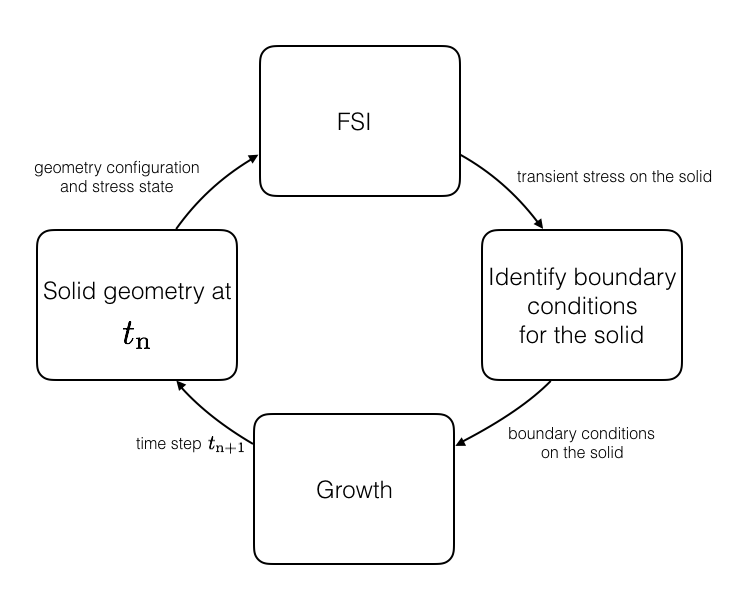
\includegraphics[width=.6\textwidth]{./figures/smallOnLarge.png} % requires the graphicx package
   \caption{Iteration and the information passing in the theory of small on large}
   \label{fig:smallOnLarge}
\end{figure}

The effect of the fluid on the solid is classified as the hydrostatic pressure $p(\bX)$ and wall shear stress $\tau(\bx)$ which are functions of the undeformed coordinates $\bX$. Let $T$ be the computational period of the FSI process, the average pressure $\bar{p}(\bX)$ and wall shear stress $\bar{\boldsymbol{\tau}}(\bX)$ can be obtained as:
\begin{subequations}
\begin{align}
\bar{p}(\bX) &= \frac{1}{T}\int_0^T p(\bX) dt\\
\bar{\boldsymbol{\tau}}(\bX) &= \frac{1}{T}\int_0^T \boldsymbol{\tau}(\bX) dt
\end{align}
\end{subequations}